\section{Localized schobers on a disc}\label{section:localized}
In this section we will define localized perverse schobers on a disc. We note that we will make no reference to non-localized schobers until \S\ref{section:adjaut}.

\begin{defn}\label{defn:compatible}
    Let $\Phi=\langle\Phi_1,\dots,\Phi_n\rangle$ be a category equipped with a right-admissible SOD $\frakS$. An autoequivalence $T$ of $\Phi$ is said to be conjugate-compatible with $\frakS$ if the composition
    \[\Phi_j\xto{I_j}\langle\Phi_1,\dots,\Phi_n\rangle\xto{T}\langle\Phi_1,\dots,\Phi_n\rangle\xto{I_i^R}\Phi_i\]
    is zero whenever $i<j$, and invertible whenever $i=j$.
\end{defn}

We point out a symmetry in this definition with the observation that the composition
\[\Phi_j\xto{I_j}\langle\Phi_1,\dots,\Phi_n\rangle\xto{I_i^R}\Phi_i\]
is zero whenever $i>j$ and identity when $i=j$.

\begin{defn}\label{defn:localized2}
    An abstract localized schober on a disc with $n$ singularities is a triple $(\frakS;\Phi,T)$ where $\Phi$ is a stable $\infty$-category, $\frakS$ is an SOD of $\Phi$, and $T$ is an autoequivalence of $\Phi$ such that $T$ is conjugate-compatible with $\frakS$.
\end{defn}

We temporarily denote the collection of abstract localized schobers on a disc with $n$ singularities by $\sfAut(n)$ and also write $\sfAut = \sfAut(1)$. We will write $\FS_{\sfAut}:\sfAut(n)\to\sfAut$ for the forgetful map
\[(\frakS;\Phi,T)\mapsto (\Phi,T).\]
This will be compatible with the ``enhanced Fukaya--Seidel functor'' which we define in \S\ref{section:adjaut}.

\begin{rmk}
    Definition~\ref{defn:localized2} needs no functorial cones, and in fact makes sense for non-stable settings. This suggests that our theory of localized schobers admits a classical counterpart in terms of triangulated categories, as well as a non-linear counterpart. Similar phenomena have been observed in \cite{kapranovPerverseSchobers2015}*{Remark 3.6}, with the notion of spherical pair, and more generally perverse schobers on a real hyperplane arrangement.
\end{rmk}

\begin{eg}\label{eg:waldhausen1}
    Let $F:\calA\tofrom \calB:G$ be a spherical adjunction and $n\geq 1$. It is shown in \cite{christGinzburgAlgebrasTriangulated2022}*{Lemma 3.8} that one can construct from this a new spherical adjunction,
    \[F':S_{n-1}(F)\tofrom \calB^{\oplus n}:G',\]
    where $S_{n-1}(F)$ is a term in the relative Waldhausen construction of \cite{dyckerhoffSphericalAdjunctionsStable2021}, and where $F',G'$ are described by explicit formulae. The category $S_{n-1}(F)$ admits an $n$-term SOD $\frakS$ of the form
    \[S_{n-1}(F) \simeq \langle\calA,\calB,\dots,\calB\rangle.\]

    In this situation, $T' := \coCone(1\to F'G')$ is conjugate-compatible with $\frakS$, and so $(\frakS;S_{n-1}(F),T')$ defines an object of $\sfAut(n)$. In Example~\ref{eg:waldhausen2}, we will explain that this actually comes from a schober with $n$ singularities.
\end{eg}

In \S\ref{subsection:comparison}, we show that this definition decategorifies to localized perverse sheaves as studied in \cite{gelfandPerverseSheavesQuivers1996}.

In \S\ref{subsection:simplicialend} and \S\ref{subsection:simplicialaut}, we will upgrade $\sfAut(n)$ to a $\two$-category, $\FS_{\sfAut}$ to a functor of $\two$-categories, and the assignment
\[\sfAut(-):[n]\mapsto\sfAut(n)\]
to a simplicial $\two$-category in such a way that the unique active map $[1]\to [n]$ induces $\FS_{\sfAut}$. More generally, the degeneracy maps $s_{n,i}:\sfAut(n)\to\sfAut(n+1)$ insert a zero into the SOD between $\Phi_i$ and $\Phi_{i+1}$, the inert face maps $d_{n,0},d_{n,n}:\sfAut(n)\to\sfAut(n-1)$ are given by forgetting $\Phi_1,\Phi_n$ respectively, and the active face maps $d_{n,i}$ merge $\Phi_i,\Phi_{i+1}$ in the SOD. We will prove that $\sfAut(n)$ is 2-Segal, which we loosely interpret as saying that localized schobers have good factorization properties.

In \S\ref{subsection:admissible}, we will prove the following recharacterization of abstract localized schobers.

\begin{thm}\label{thm:alternate}
    Let $\Phi$ be a stable category equipped with a right-admissible SOD $\frakS$ and autoequivalence $T$. Then, $(\Phi,\frakS,T)$ is an abstract localized schober if and only if $\frakS$ is $\infty$-admissible, and
    \[T(\frakS) = \delta^{-2}\cdot \frakS,\]
    where $T(\frakS)$ is the result of applying $T$ to each subcategory, and $\delta^2 \in\Br_n$ is the positive full-twist element.
\end{thm}

The infinite admissibility lets us construct an action of the braid group $\Br_n$ on the $\two$-category $\sfAut(n)$. We will use this to define $\two$-categories of non-abstract localized perverse schobers, denoted $\olsftwoP(\bbC,R)$, where $R\subset\bbC$ is a finite subset.

In \S\ref{subsection:interpretation}, we conclude the section by giving two related interpretations of localized schobers, the first in terms of Serre functors and the second in terms of the global monodromy of the Fukaya--Seidel category of a Lefschetz fibration.

\subsection{Comparison to localized perverse sheaves}\label{subsection:comparison}
We compare the definition of abstract localized schobers with that of localized perverse sheaves. We recall the following.

\begin{prop}[Gelfand--MacPherson--Vilonen, \cite{gelfandPerverseSheavesQuivers1996}*{Proposition 2.3}]\label{prop:gmvquiver}
    Let $R\subset \bbC$ a finite subset of size $n$. Let $K_n$ be the quiver with $n$ vertices and arrows $j\to i$ for all $1\leq i,j\leq n$. Let $\opname{Q}(n)$ be the category of quiver representations $(M_i,m_{ij})$ of $K_n$ such that for all $i$, $1-m_{ii}$ is invertible.

    After making a choice of cuts on $(\bbC,R)$, there is an equivalence of categories,
    \[\Perv(\bbC,R)/\Loc(\bbC)\simeq \opname{Q}(n).\]
\end{prop}

We unravel the definition of abstract localized schober to resemble this quiver description. Recall that by the theory of gluing functors (which arises here as the monadicity of $\oplus_iI_i^R$), the data of the SOD $\Phi=\langle\Phi_1,\dots,\Phi_n\rangle$ is equivalent to giving the components $\Phi_i$, together with gluing functors $F_{ij} := I_i^RI_j$ and its monad structure. By orthogonality, $F_{ij}=0$ when $i>j$, so this monad is upper triangular. Moreover $F_{ii}\simeq 1$. This can be seen as the ``upper triangular half'' of the categorical quiver representation.

The ``lower triangular half'' comes from the autoequivalence $T$. Define $T_{ij} := I_i^RTI_j:\Phi_j\to \Phi_i$. Conjugate-compatibility says that $T_{ij}=0$ when $i<j$ and that $T_{ii}$ is invertible. This collection of functors admits a ``bimodule structure'' for the lower triangular monad $F := (F_{ij})_{i\leq j}$. We see that the data of the functor $T$ is equivalent to the functors $(T_{ij})_{i\leq j}$ together with its bimodule structure. So we have the following.

\begin{prop}\label{prop:decategorification1}
    Given an abstract localized perverse schober $(\Phi,\Phi_i,T)\in\sfAut(n)$, we may form an object of $\opname{Q}(n)$ by taking $M_i := K_0(\Phi_i)$ and $m_{ij} = K_0(F_{ij}\oplus T_{ij})$.
\end{prop}

\begin{rmk}
    Additional structures such as the monad structure and the bimodule structure disappear when we decategorify, as these are encoded by 2-morphisms in $\sfSt_k$. In plain terms, if $f,g:V\to W$ are linear maps of vector spaces, we can't make sense of a (non-invertible) morphism $f\to g$.
\end{rmk}

\subsection{\texorpdfstring{$\sfEnd(n)$}{End(n)} as a simplicial \texorpdfstring{$\two$}{2}-category}\label{subsection:simplicialend}

We will consider a variant of $\sfAut(n)$ where we don't impose invertibility conditions, and construct out of this a simplicial $\two$-category.

\begin{defn}
    Let $\Phi$ be a category equipped with a (possibly partial) SOD $\frakS=(\Phi_1,\dots,\Phi_n)$. Denote by $I_i$ the inclusion functors. An \textit{endofunctor} $T$ of $\Phi$ is said to be weakly conjugate-compatible with $\frakS$ if the composition
    \[\Phi_j\xto{I_j}\langle\Phi_1,\dots,\Phi_n\rangle\xto{T}\langle\Phi_1,\dots,\Phi_n\rangle\xto{I_i^R}\Phi_i\]
    is zero whenever $i<j$.
\end{defn}

\begin{notn}
    We denote by $\sfEnd$ the $\two$-category of pairs $(\Phi,T)$ where $T:\Phi\to\Phi$ is an endofunctor. We denote by $\sfEnd(n)$ the $\two$-category of data $(\Phi,\frakS,T)$ where $\Phi$ is a category, $\frakS$ is an SOD of $\Phi$, and $T:\Phi\to\Phi$ is an \textit{endofunctor}, weakly conjugate-compatible with $\frakS$. These $\two$-categories are constructed similarly to $\sfAut(n)$.
\end{notn}

We upgrade the assignment $[n]\mapsto \sfEnd(n)$ to a simplicial $\two$-category which is 2-Segal. Consider the simplicial $\two$-category
\[[n]\mapsto \sfSOD'(n)\times_{\sfSt_k}\sfEnd,\]
where the functors to $\sfSt_k$ are given by $\opname{U}:\sfSOD'(n)\to\sfSt_k$, and $\sfEnd\to\sfSt_k$ is the forgetful functor. We denote objects by $(\Phi_1,\dots,\Phi_n;\Phi,T)$ and write $I_i:\Phi_i\inclto \Phi$ for inclusions of subcategories.

Define the sub-$\two$-category
\[\sfEnd'(n)\subseteq \sfSOD'(n)\times_{\sfSt_k}\sfEnd\]
consisting of those objects $(\frakS;\Phi,T)$ for which the endofunctor $T$ is weakly conjugate-compatible with the partial SOD $\frakS$ of $\Phi$.

\begin{prop}\label{prop:segalend}
    The assignment $\sfEnd'(-):[n]\mapsto \sfEnd'(n)$ is a simplicial sub-$\two$-category of $\sfSOD'(-)\times_{\sfSt_k}\sfEnd$. Moreover, $\sfEnd'(-)$ is 2-Segal.
\end{prop}

\begin{proof}
    We show that $\sfEnd'(n)$ maps to $\sfEnd'(n-1)$ under the face maps $d_{n,i}$ for $0<i<n$. Stability under the remaining face maps and degeneracy maps is easy to verify.

    Let $(\Phi_1,\dots,\Phi_n;\Phi,T)\in \sfEnd'(n)$. The operation $d_{n,i}$ collapses $\Phi_i,\Phi_{i+1}$ into $\langle\Phi_i,\Phi_{i+1}\rangle$, whose inclusion we denote by $I_{i,i+1}$. So we must verify that for all $j>i+1$,
    \[I_{i,i+1}^R T I_{j} = 0\]
    and that for all $j<i$,
    \[I_j^R T I_{i,i+1} = 0.\]
    The first of these follows by post-composing with $\langle\Phi_i,\Phi_{i+1}\rangle\to \Phi_i\oplus\Phi_{i+1}$ which is conservative. The second of these follows because $\langle\Phi_i,\Phi_{i+1}\rangle$ is generated by $\Phi_i$ and $\Phi_{i+1}$.

    We now verify the 2-Segal condition. By Proposition~\ref{prop:segalsod}, $\sfSOD'(n)$ is 2-Segal. It follows that for each square in $\Delta$ as in (\ref{equation:twosegal}), the natural map
    \[\sfEnd'(n)\to \sfEnd'(m)\times_{\sfEnd'(1)}\sfEnd'(n+1-m)\]
    is 2-fully faithful. So we can work on the level of objects as follows.
    
    Let $(\Phi_1,\dots,\Phi_n;\Phi,T)\in \sfSOD'(-)\times_{\sfSt_k}\sfEnd$. Given $0<i<j<n$, suppose that
    \[(\Phi_i,\dots,\Phi_j;\Phi,T), (\Phi_1,\dots,\Phi_{i-1},\Phi_{i,\dots,j},\Phi_{j+1},\dots,\Phi_n;\Phi,T)\]
    individually lie in $\sfEnd'(-)$. Here, $\Phi_{i,\dots,j} := \langle\Phi_i,\dots,\Phi_j\rangle$, and we write $I_{i,\dots,j}$ for its inclusion as a subcategory inside $\Phi$. It will suffice to prove that $(\Phi_1,\dots,\Phi_n;\Phi,T)$ also lies in $\sfEnd'(-)$.

    We must verify that for all $1\leq i' < j'\leq n$, $I_{i'}^RTI_{j'}=0$. If both $i',j'$ lie inside $\{i,\dots,j\}$ or if they both lie outside $\{i,\dots,j\}$, then this is clear. If just $j'$ lies inside then $I_{j'}$ factors as $\Phi_{j'}\xto{I_{j'}^{i,\dots,j}} \Phi_{i,\dots,j}\xto{I_{i,\dots,j}} \Phi$, so
    \[I_{i'}^RTI_{j'} = I_{i'}^RTI_{i,\dots,j}I_{j'}^{i,\dots,j}  = 0.\]
    The argument is similar if just $i'$ lies in $\{i,\dots,j\}$ so we are done.
\end{proof}

For each $n$, there is an inclusion functor, $\opname{I}_n:\sfEnd(n) \inclto \sfEnd'(n)$ identifying $\sfEnd(n)$ with the full sub-$\two$-category of those objects where the partial SOD is an SOD.

\begin{lem}\label{lem:rightadjointend}
    The inclusion functor $\opname{I}_n:\sfEnd(n) \inclto \sfEnd'(n)$ admits a right adjoint $\opname{I}_n^R$, which is given on objects by
    \[(\frakS;\Phi,T)\mapsto (\frakS;\langle\Phi_1,\dots,\Phi_n\rangle,I^RTI),\]
    where $I:\langle\Phi_1,\dots,\Phi_n\rangle\inclto \Phi$.
\end{lem}

\begin{proof}
    Consider first the case $n=1$. Then, the right adjoint exists and is given on objects by
    \[(\Phi_1;\Phi,T)\mapsto (\Phi_1,I_1^RTI_1),\]
    by a proof similar to that of Lemma~\ref{lem:keyrightadjoint}.

    For general $n$, consider the following commuting diagram of $\two$-categories, where each arrow is 2-fully faithful.
    \[\begin{tikzcd}[ampersand replacement=\&]
        {\sfEnd(n)} \& {\sfEnd'(n)} \\
        {\sfSOD(n)\times_{\sfSt_k}\sfEnd(1)} \& {\sfSOD(n)\times_{\sfSt_k}\sfEnd'(1)}
        \arrow["{\opname{I}_n}", hook, from=1-1, to=1-2]
        \arrow[hook, from=1-1, to=2-1]
        \arrow[hook, from=1-2, to=2-2]
        \arrow["{\id\times\opname{I_1}}"', hook, from=2-1, to=2-2]
    \end{tikzcd}\]
    The bottom horizontal arrow has a right adjoint by the case $n=1$. This right adjoint preserves the full sub-$\two$-categories, and hence induces a right adjoint of $\opname{I}_n$, given by the formula in the statement.
\end{proof}

\begin{cor}\label{prop:simplicialend}
    The assignment $[n]\mapsto\sfEnd(n)$ upgrades to a simplicial $\two$-category. For $0\leq i\leq n$, the degeneracy map
    \[s_{n,i}:\sfEnd(n)\to \sfEnd(n+1)\]
    inserts a $0$ between $\Phi_i$ and $\Phi_{i+1}$. For $0< i< n$, the active face map
    \[d_{n,i}:\sfEnd(n)\to \sfEnd(n-1)\]
    merges $\Phi_i,\Phi_{i+1}$ into $\langle\Phi_i,\Phi_{i+1}\rangle$. The inert face maps $d_{n,0}$ and $d_{n,n}$ remove $\Phi_1$ and $\Phi_n$ respectively. 

    The assignment $[n]\mapsto \sfEnd(n)$ upgrades to a simplicial $\two$-category. For $0\leq i\leq n$, the degeneracy map $s_{n,i}$ inserts a $0$ between $\Phi_i$ and $\Phi_{i+1}$;
    \begin{align*}
        s_{n,i}:\sfEnd(n)&\to\sfEnd(n+1)\\
        (\frakS;\Phi,T)&\mapsto ((\Phi_1,\dots,\Phi_i,0,\Phi_{i+1},\dots\Phi_n);\Phi,T).
    \end{align*}
    The inert face map $d_{n,0}$ removes $\Phi_1$ from the SOD to get $\Phi_{2,\dots,n} := \langle\Phi_2,\dots,\Phi_n\rangle\xto{I_{2,\dots,n}}\Phi$;
    \begin{align*}
        d_{n,0}:\sfEnd(n)&\to\sfEnd(n-1)\\
        (\frakS;\Phi,T)&\mapsto ((\Phi_2,\dots,\Phi_n);\Phi_{2,\dots,n},I_{2,\dots,n}^RTI_{2,\dots,n}),
    \end{align*}
    and the other inert face map $d_{n,n}$ similarly removes $\Phi_n$ from the SOD. For $0<i<n$, the active face map is given by merging $\Phi_{i}$ and $\Phi_{i+1}$ in the SOD into $\Phi_{i,i+1} := \langle\Phi_i,\Phi_{i+1}\rangle$;
    \begin{align*}
        d_{n,i}:\sfEnd(n)&\to\sfEnd(n-1)\\
        (\frakS;\Phi,T)&\mapsto ((\Phi_1,\dots,\Phi_{i-1},\Phi_{i,i+1},\Phi_{i+2},\dots\Phi_n);\Phi,T).
    \end{align*}
\end{cor}

\begin{proof}
    We apply Lemma~\ref{lem:descendingsimplicialobjects}. We omit the verification that the resulting lax-commuting squares are commuting squares.
\end{proof}

\begin{prop}
    The simplicial $\two$-category $\sfEnd(-)$ is 2-Segal.
\end{prop}

\begin{proof}
    The strategy used in the proof of Proposition~\ref{prop:segalsod} works by observing that the map $\sfEnd'(-)\to\sfEnd(-)$ is Cartesian over $\Delta_{\act}$.
\end{proof}

\subsection{\texorpdfstring{$\sfAut(n)$}{Aut(n)} as a simplicial \texorpdfstring{$\two$}{2}-category}\label{subsection:simplicialaut}
We now reinstate the invertibility conditions and construct the $\two$-category of abstract localized schobers, and upgrade this to a simplicial $\two$-category which is 2-Segal.

\begin{notn}
    We denote by $\sfAut$ the $\two$-category of data $(\Phi,T)$ consisting of a stable category equipped with an autoequivalence. This admits a forgetful functor, $\sfAut\to\sfSt_k$. We denote by $\sfAut(n)$ the full sub-$\two$-category of $\sfAut\times_{\sfSt_k}\sfSOD(n)$ of abstract localized schobers.
\end{notn}

We now exhibit $[n]\mapsto \sfAut(n)$ as a 2-Segal simplicial $\two$-category.

\begin{prop}\label{prop:simplicialaut}
    The full sub-$\two$-categories $\sfAut(n)\inclto \sfEnd(n)$ form a sub-simplicial $\two$-category which is also 2-Segal.
\end{prop}

We begin with two technical lemmas.
\begin{lem}\label{lem:technical}
    Let $\Phi$ be a category, and $\frakS=(\Phi_1,\Phi_2)$ be a right-admissible SOD. Let $T:\Phi\to \Phi$ be an autoequivalence such that $I_1^RTI_2=0$. Write $T_i := I_i^RTI_i$. If $T_1$ is invertible, then there is a natural identification,
    \[\Cone(I_2I_2^{R}\to \id)\simeq I_1T_1^{-1}I_1^RT.\]
    If $T_2$ is invertible, then there is a natural identification,
    \[\Cone(I_1I_1^{R}\to \id)\simeq TI_2T_2^{-1}I_2^R.\]
\end{lem}

\begin{proof}
    Let us prove the second statement. Consider the diagram of functors
    \[\id\from I_2I_2^R\to TI_2T_2^{-1}I_2^R,\]
    where the first arrow is the counit and the second comes from $\id \simeq I_2^RTI_2(T_2^{-1})$. We postcompose the diagram by $I_1I_1^R\to \id$ to obtain the following commuting diagram.
    \[\begin{tikzcd}[ampersand replacement=\&]
	{I_1I_1^R} \& {I_1I_1^RI_2I_2^R} \& 0 \\
        \id \& {I_2I_2^R} \& {TI_2T_2^{-1}I_2^R}
        \arrow[from=1-1, to=2-1]
        \arrow[from=1-2, to=1-1]
        \arrow[from=1-2, to=1-3]
        \arrow[from=1-2, to=2-2]
        \arrow[from=1-3, to=2-3]
        \arrow[from=2-2, to=2-1]
        \arrow[from=2-2, to=2-3]
    \end{tikzcd}\]
    The top right is zero by $I_1^RTI_2=0$. The left square is Cartesian by Lemma~\ref{lem:SODcharacterizations}. The right square is also Cartesian because if we apply either $I_1^R$ or $I_2^R$, it becomes Cartesian. It follows that the cones of the vertical maps all agree, giving the desired identification.

    The first statement is similar beginning with
    \[\id\from I_1I_1^R\to I_1T_1^{-1}I_1^RT,\]
    and precomposing with $I_2I_2^R\to \id$.
\end{proof}

\comment{
    \begin{proof}
        Let us prove the second statement. Consider the functor
        \[H := \coCone(I_2T_2\to TI_2),\]
        where the map shown comes is the counit map for $I_2\adjto I_2^R$. It follows that $I_2^RH = 0$, and therefore $H$ factors through $\Phi_1$. So we have an identification,
        \[H \isomfrom I_1I_1^R\coCone(I_2T_2\to TI_2) \simeq I_1I_1^RI_2T_2,\]
        where the second identification uses that $I_1^RTI_2=0$. We thus have an exact triangle,
        \[I_1I_1^RI_2T_2\to I_2T_2 \to TI_2\xto{+1}.\]
        Moving things around, we obtain the exact triangle,
        \begin{equation}\label{equation:1}
            I_1I_1^RI_2I_2^R\to I_2I_2^R \to TI_2T_2^{-1}I_2^R\xto{+1}.
        \end{equation}
        Now, by Lemma~\ref{lem:SODcharacterizations} applied to $\frakS$, we have that
        \[\Cone(I_1I_1^{R}\to 1)\Cone(I_2I_2^{R}\to 1)=0,\]
        so that
        \begin{equation}\label{equation:2}
            \Cone(I_1I_1^{R}\to 1)\simeq \Cone(I_1I_1^{R}\to 1)I_2I_2^{R}.
        \end{equation}
        Putting (\ref{equation:1}) and (\ref{equation:2}) together, we have
        \[\Cone(I_1I_1^{R}\to 1)\simeq TI_2T_2^{-1}I_2^R.\]

        The first statement is similar. We begin by considering the functor
        \[K = \coCone(T_1I_1^R\to I_1^RT).\]
        Now, $KI_1=0$ so that $K$ vanishes on $\Phi_1$. Moreover, the image of $\Cone(I_2I_2^R\to 1)$ lies in $\Phi_1$, so we have an identification
        \[K\simeq KI_2I_2^R,\]
        and subsequently an exact triangle,
        \[T_1I_1^RI_2I_2^R\to T_1I_1^R\to I_1^RT\xto{+1}.\]
        By moving things around, we deduce that
        \[I_1I_1^R\Cone(I_2I_2^{R}\to 1)\simeq I_1T_1^{-1}I_1^RT,\]
        hence by Lemma~\ref{lem:SODcharacterizations} applied to $\frakS$,
        \[\Cone(I_2I_2^{R}\to 1)\simeq I_1T_1^{-1}I_1^RT.\]
    \end{proof}
}

\begin{lem}\label{lem:invertibletwo}
    Let $\Phi$ be a category, and $\frakS=(\Phi_1,\Phi_2)$ be a right-admissible SOD. Let $T:\Phi\to \Phi$ be an autoequivalence such that $I_1^RTI_2=0$. Write $T_i := I_i^RTI_i$. Then, $T_1$ is an autoequivalence if and only if $T_2$ is an autoequivalence.
\end{lem}

\begin{proof}
    Suppose that $T_1$ is an autoequivalence. We claim that
    \[V_2 := I_2^RT^{-1}\Cone(I_1I_1^R\to \id)I_2\]
    is an inverse to $T_2$. This is a formal but tedious verification. We have
    \begin{align*}
        V_2T_2 &= I_2^RT^{-1}\Cone(I_1I_1^R\to \id)I_2\circ I_2^RTI_2\\
        &\simeq I_2^RT^{-1}\Cone(I_1I_1^R\to \id)TI_2\\
        &\simeq I_2^RT^{-1}TI_2\\
        &\simeq \id_{\Phi_2}.
    \end{align*}
    
    To evaluate $T_2V_2$, see that
    \begin{align*}
        T_2V_2 = I_2^RTI_2\circ I_2^RT^{-1}\Cone(I_1I_1^R\to \id)I_2
    \end{align*}
    is the cone of a map between the following functors,
    \begin{align*}
        &I_2^RT \circ T^{-1}\Cone(I_1I_1^R\to \id)I_2,\\
        &I_2^RT \circ \Cone(I_2I_2^R\to \id)\circ T^{-1}\Cone(I_1I_1^R\to \id)I_2.
    \end{align*}
    The first of these is identified with $\id_{\Phi_2}$. The second is evaluated using Lemma~\ref{lem:technical} as follows.
    \begin{align*}
        &I_2^RT \circ\Cone(I_2I_2^R\to \id)\circ T^{-1}\Cone(I_1I_1^R\to \id)I_2\\
        \simeq&  I_2^RT \circ I_1T_1^{-1}I_1^RT\circ T^{-1}\Cone(I_1I_1^R\to \id)I_2\\
        \simeq& I_2^RT \circ I_1T_1^{-1}I_1^R \Cone(I_1I_1^R\to \id)I_2\\
        \simeq &0.
    \end{align*}
    So $T_2V_2\simeq \id_{\Phi_2}$.

    The proof in the other direction is similar, with inverse given by
    \[V_1 := I_1^R\Cone(I_2I_2^R\to \id)T^{-1}I_1.\]
\end{proof}

\begin{proof}[Proof of Proposition~\ref{prop:simplicialaut}]
    It is clear that the degeneracy maps and the inert face maps $d_{n,0},d_{n,n}$ preserve $\sfAut(-)$. We verify that the active face maps $d_{n,i}:\sfEnd(n)\to\sfEnd(n-1)$ for $0<i<n$ preserve $\sfAut(-)$. Recall these functors are given by
    \[(\Phi_1,\dots,\Phi_n;\Phi,T)\mapsto (\Phi_1,\dots\Phi_{i,i+1}\dots,\Phi_n;\Phi,T),\]
    where $I_{i,i+1}:\Phi_{i,i+1} \inclto \Phi$ is subcategory generated by $\Phi_i,\Phi_{i+1}$. It suffices to verify that $I_{i,i+1}^RTI_{i,i+1}$ is invertible. This follows by repeatedly applying Lemma~\ref{lem:invertibletwo}. We thus deduce that $\sfAut(-)$ is a sub-simplicial $\two$-category.

    We now verify the 2-Segal condition. Let $(\Phi_1,\dots,\Phi_n;\Phi,T)\in \sfEnd(n)$. Given $0<i<j<n$, suppose that
    \[(\Phi_i,\dots,\Phi_j;\Phi,T_{i,\dots,j}), (\Phi_1,\dots,\Phi_{i-1},\Phi_{i,\dots,j},\Phi_{j+1},\dots,\Phi_n;\Phi,T)\]
    individually lie in $\sfAut(-)$. Here, $\Phi_{i,\dots,j} := \langle\Phi_i,\dots,\Phi_j\rangle$, $I_{i,\dots,j}$ is its inclusion as a subcategory inside $\Phi$ and $T_{i,\dots,j} = I_{i,\dots,j}^RTI_{i,\dots,j}$. It will suffice to prove that $(\Phi_1,\dots,\Phi_n;\Phi,T)$ lies in $\sfAut(n)$.

    We must verify that for all $1\leq i' \leq n$, $I_{i'}^RTI_{i'}$ is invertible. If $i'$ lies outside $\{i,\dots,j\}$ then this is clear. Otherwise, $I_{i'}$ factors as $\Phi_{i'}\xto{I_{i'}^{i,\dots,j}} \Phi_{i,\dots,j}\xto{I_{i,\dots,j}} \Phi$, so
    \[I_{i'}^RTI_{i'} = (I_{i'}^{i,\dots,j})^RT_{i,\dots,j}I_{i'}^{i,\dots,j}\]
    is invertible. This completes the proof.
\end{proof}

\subsection{Braid group action on abstract localized schobers}\label{subsection:admissible}
We establish that abstract localized perverse schobers enjoy a braid group action by mutation of its SOD. We then prove Theorem~\ref{thm:alternate} which gives an alternate characterization of abstract localized schobers.

\begin{thm}\label{thm:inftyadmissible}
    Let $(\Phi,\frakS,T)\in\sfAut(n)$ be an abstract localized schober. Then, $\frakS$ is an $\infty$-admissible SOD. Moreover, for any $\beta\in\Br_n$, $(\Phi,\beta\cdot\frakS,T)$ is an abstract localized schober.
\end{thm}

\begin{cor}\label{cor:action}
    There is a natural action of the braid group $\Br_n$ on $\sfAut(n)$. Moreover, $\FS_{\sfAut}:\sfAut(n)\to\sfAut$ is naturally $\Br_n$-equivariant where $\sfAut$ is given the trivial action.
\end{cor}

\begin{proof}
    It follows from Lemma~\ref{lem:Uisfaithful} that $\FS_{\sfAut}:\sfAut(n)\to\sfAut$ is 2-faithful. So functors $\sfAut(n)\to \sfAut(n)$ over $\sfAut$ may be defined at the level of objects by Proposition~\ref{prop:functorconstruction}. Using this, we can check that for each $\beta\in\Br_n$, the assignment of Theorem~\ref{thm:inftyadmissible} extends to a functor
    \[\mathop{A}(\beta): \sfAut(n)\to\sfAut(n),\]
    and so we obtain a functor of $\one$-categories,
    \begin{align*}
        \Br_n&\to \Hom_{(\wCat_{\two})_{/\sfAut}}(\sfAut(n),\sfAut(n))\\
        \beta&\mapsto \mathop{A}(\beta).
    \end{align*}
    
    To extend this to a group action, we must lift this to a monoidal functor. It follows by Proposition~\ref{prop:functorconstruction} that the target $\one$-category is in fact discrete, so it is a property for this functor to be monoidal. This amounts to checking that the functors $\mathop{A}(\beta_1)\circ \mathop{A}(\beta_2)$ and $\mathop{A}(\beta_1\beta_2)$ agree at the level of objects, which in turn follows from Lemma~\ref{lem:relations}.
\end{proof}

We begin by studying the smallest non-trivial case of Theorem~\ref{thm:inftyadmissible}.
\begin{lem}\label{lem:nistwo}
    Theorem~\ref{thm:inftyadmissible} holds for $n=2$.
\end{lem}

\begin{proof}
    Let $\sigma_1\in\Br_2$ be the positive generator. By induction on the length of the braid group element, it suffices to verify the following.
    \begin{enumerate}
        \item $\frakS$ admits a mutation by $\sigma_1$, and $T$ is conjugate-compatible with $\sigma_1\cdot\frakS$.
        \item $\frakS$ admits a mutation by $\sigma_1^{-1}$, and $T$ is conjugate-compatible with $\sigma_1^{-1}\cdot\frakS$.
    \end{enumerate}

    We will prove the second statement. We write $\frakS=(\Phi_1,\Phi_2)$ and $I_i:\Phi_i\inclto\Phi$ as usual. Write also,
    \[T_i := I_iTI_i^R,\]
    which we recall is an autoequivalence of $\Phi_i$. We show that the subcategories $(T(\Phi_2),\Phi_1)$ define a right-admissible SOD of $\Phi$, thereby exhibiting the mutation $\sigma_1^{-1}\cdot\frakS$. It is clear that the inclusion functors $I_1' := TI_2, I_2' := I_1$ admit right adjoints, and that we have semi-orthogonality,
    \[I_2'^{R}I_1' = I_1^RTI_2=0.\]
    By Lemma~\ref{lem:SODcharacterizations}, it suffices to show that
    \[\Cone(I_1'I_1'^{R}\to \id)\Cone(I_2'I_2'^{R}\to \id)=0.\]
    By Lemma~\ref{lem:technical},
    \[\Cone(I_2'I_2'^{R}\to \id)\simeq I_1'T_2^{-1}I_1'^RT^{-1}.\]
    We deduce therefore that
    \[\Cone(I_1'I_1'^{R}\to \id)\Cone(I_2'I_2'^{R}\to \id) = 0.\]

    Let us now verify that $T$ is conjugate-compatible with the mutation $\sigma_1\cdot\frakS$. We see that $I_1'^RTI_2' \simeq I_2^RI_1=0$, and also that $I_1'^RTI_1' \simeq T_2$, $I_2'^RTI_2' \simeq T_1$ are invertible, as required.

    The first statement is proven similarly, starting with the claim that the list of subcategories $(\Phi_2,T^{-1}(\Phi_1))$ defines the mutation by $\sigma_1$.
\end{proof}

In order to prove Theorem~\ref{thm:inftyadmissible} for general $n$, we will take advantage of the 2-Segal property of $\sfAut(-)$.

\begin{proof}[Proof of Theorem~\ref{thm:inftyadmissible}]
    We show that for each $i=1,\dots,n-1$ and sign $\epsilon\in\{1,-1\}$, $\frakS$ admits a mutation by $\sigma_i^{\epsilon}$, and $T$ is conjugate-compatible for the mutation $\sigma_i^{\epsilon}\cdot\frakS$.

    From the 2-Segal property of $\sfAut(-)$ which was proven in Proposition~\ref{prop:simplicialaut}, we have a pullback square as follows.
    \[\begin{tikzcd}[ampersand replacement=\&]
        {\sfAut(n)}\pullback \& {\sfAut(2)} \\
        {\sfAut(n-1)} \& {\sfAut(1)}
        \arrow[from=1-1, to=1-2]
        \arrow[from=1-1, to=2-1]
        \arrow[from=1-2, to=2-2]
        \arrow[from=2-1, to=2-2]
    \end{tikzcd}\]
    Here, the top horizontal arrow restricts to the 2-term SOD comprised of $\Phi_i,\Phi_{i+1}$, and the left vertical arrow contracts these two components. The relevant mutation on $\sfAut(2)$ induces via this pullback square, the desired mutation.
\end{proof}

We conclude by proving Theorem~\ref{thm:alternate}, which provides an alternate characterization of abstract localized schobers.

\begin{proof}[Proof of Theorem~\ref{thm:alternate}]
    Suppose that $(\Phi,\frakS,T)$ is an abstract localized schober. Then by Theorem~\ref{thm:inftyadmissible}, $\frakS$ is $\infty$-admissible. We verify that $T(\frakS) = \delta^{-2}\cdot \frakS$. Generalizing the proof of Lemma~\ref{lem:nistwo}, we see that
    \[\tau^{-1}\cdot\frakS = (T(\Phi_n),\Phi_1,\Phi_2,\dots,\Phi_{n-1})\]
    where $\tau = \sigma_{n-1}\cdots\sigma_1$ is one of the positive cyclic rotations. This is illustrated below for $n=5$. Since $\tau^n = \delta^2$, we are done.
    \[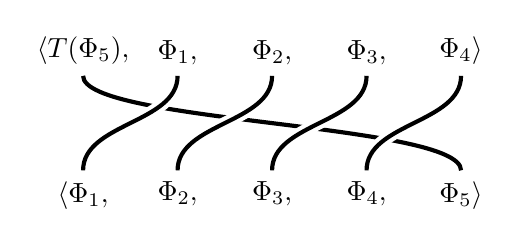
\begin{tikzpicture}[scale=1.2]
        % Strand style definitions
        \tikzset{
            strand/.style={black, line width=1.5pt},
            mask/.style={white, line width=4.5pt}
        }

        % ==========================================
        % TOP BRAID (y = 1 to y = 0)
        % ==========================================
        % Background strand:
        \draw[strand] (5, 0) .. controls (5, 0.5) and (1,0.5) .. (1, 1) node[at start, below] {$\Phi_5\rangle$} node[above, black] {$\langle T(\Phi_5),$} ;

        % Foreground strands
        \draw[mask] (1, 0) .. controls (1, 0.5) and (2,0.5) .. (2, 1);
        \draw[mask] (2, 0) .. controls (2, 0.5) and (3,0.5) .. (3, 1);
        \draw[mask] (3, 0) .. controls (3, 0.5) and (4,0.5) .. (4, 1);
        \draw[mask] (4, 0) .. controls (4, 0.5) and (5,0.5) .. (5, 1);
        \draw[strand] (1, 0) .. controls (1, 0.5) and (2,0.5) .. (2, 1) node[at start, below] {$\langle\Phi_1,$} node[above, black] {$\Phi_1,$};
        \draw[strand] (2, 0) .. controls (2, 0.5) and (3,0.5) .. (3, 1) node[at start, below] {$\Phi_2,$} node[above, black] {$\Phi_2,$} ;
        \draw[strand] (3, 0) .. controls (3, 0.5) and (4,0.5) .. (4, 1) node[at start, below] {$\Phi_3,$} node[above, black] {$\Phi_3,$} ;
        \draw[strand] (4, 0) .. controls (4, 0.5) and (5,0.5) .. (5, 1) node[at start, below] {$\Phi_4,$} node[above, black] {$\Phi_4\rangle$} ;
    \end{tikzpicture}\]

    We now prove the converse. For each $i$, let $\Phi_i'$ be the right-orthogonal of $\oplus_{j\neq i}\Phi_j$. These subcategories have the property that $I_i^R$ is zero on $\Phi_{j}$ for $j\neq i$ and induces an equivalence on $\Phi_i'$. These are the subcategories that form the mutation,
    \[\delta^{-1}\cdot\frakS := (\Phi_n',\dots,\Phi_1').\]
    where for example, $\Phi_1' = \Phi_1$. 
    
    Now by assumption, $T(\Phi_n) = \Phi_n'$. By the property above, $I_i^RTI_n = 0$ for all $i<n$, and is an equivalence for $i=n$.

    Next, observe that as subcategories of $\Phi$,
    \[\langle T(\Phi_{n-1}),T(\Phi_n)\rangle = \langle \Phi_n',\Phi_{n-1}'\rangle.\]
    So by the property above, $I_i^RTI_{n-1} = 0$ for all $i<n-1$, and is an equivalence for $i=n-1$. Continuing in this fashion, we deduce that $T$ is conjugate-compatible for $\frakS$, as desired.
\end{proof}

Let $R\subset\bbC$ be a finite subset. We define non-abstract localized schobers on $(\bbC,R)$ by using the braid group action and a $\two$-categorical version of the construction in \cite{kapranovPerverseSchobers2015}. 

\begin{defn}\label{defn:cuts}
    A system of cuts $K$ on $(\bbC,R)$ is a choice of arcs connecting the points of $R$ to a point $\infty\in\bbC$ far away on the positive real axis. We let $\Cuts(\bbC,R)$ denote the space of systems of cuts. 
\end{defn}

The space $\Cuts(\bbC,R)$ is a torsor under a homotopical right action by the group $\Br_n$, acting by mutations of cuts, see \cite{kapranovPerverseSchobersAlgebra2020}*{Figure 8}.

Consider now the trivial local system $\ul{\sfAut}(n)$ of $\two$-categories over $\Cuts(\bbC,R)$ where each stalk is given by $\sfAut(n)$. The action of $\Br_n$ on $\sfAut(n)$ upgrades $\ul{\sfAut}(n)$ to a $\Br_n$-equivariant local system.

\begin{defn}\label{defn:nonabstract}
    We let $\olsftwoP(\bbC,R)$ be the $\two$-category of sections of $\ul{\sfAut}(n)$ that are invariant under $\Br_n$, and refer to an object of $\sftwoP(\bbC,R)$ as a localized perverse schober on $(\bbC,R)$.
\end{defn}

\subsection{Serre functors and global monodromy}\label{subsection:interpretation}
We relate our notion of abstract localized schobers to Serre functors on the one hand, and to the global monodromy of the Fukaya--Seidel category of a Lefschetz fibration on the other.

\begin{eg}\label{eg:aut2}
    We give a more explicit description of objects in $\sfAut(2)$. Recall from \cite{dyckerhoffSphericalAdjunctionsStable2021}*{Corollary 2.5.3} that a 2-term $\infty$-admissible SOD $\langle\calA,\calB\rangle$, is equivalent to a diagram $F:\calB\to\calA$ of categories where $F$ admits all adjoints. The mutation of this SOD by the full twist is abstractly given by the diagram $F^{RR}:\calB\to\calA$. Thus a conjugate-compatible autoequivalence $T$ is equivalent to the data of autoequivalences $T_\calA,T_\calB$ of $\calA$, $\calB$ respectively, together with an equivalence, $F\circ T_\calB\simeq T_{\calA}\circ F^{RR}$.

    A source of such objects come from Serre functors. Let $\calA = \QCoh(X),\calB = \QCoh(Y)$ where $X$ and $Y$ are smooth projective varieties over $k$. Let $\omega_X := \pi_X^!k$ denote the shifted dualizing sheaf on $X$ and $\omega_Y$ likewise, so that
    \[T_\calA := -\otimes\omega_X^{-1},T_\calB := -\otimes\omega_Y^{-1}\]
    are the inverse Serre functors. Let $F = f^*$ for some smooth morphism $f:X\to Y$. Then by Grothendieck duality, this gives an object of $\sfAut(2)$.
\end{eg}

An algebraic relationship between $\delta^2$ and the Serre functor generalizing Example~\ref{eg:aut2} can be found in \cite{kapranovPerverseSchobersAlgebra2020}.

\begin{prop}\label{prop:serrefunctor}
    Suppose that $\Phi$ admits a Serre functor $S$. Then, for any right-admissible SOD $\frakS$ of $\Phi$, $(\frakS;\Phi,S^{-1})$ is an abstract localized schober.
\end{prop}

\begin{proof}
    By \cite{kapranovPerverseSchobersAlgebra2020}*{Proposition 3.3.5}, $\frakS$ is $\infty$-admissible. By \cite{kapranovPerverseSchobersAlgebra2020}*{Proposition 3.3.11},
    \[\delta^2\cdot\frakS = S(\frakS),\]
    so we are done by Theorem~\ref{thm:alternate}.
\end{proof}

In this way, we can think of the characterization of Theorem~\ref{thm:alternate} as saying that $(\Phi,\frakS,T)$ is an abstract localized schober whenever $T$ behaves like an inverse Serre functor with respect to the SOD $\frakS$. We can find related observations in earlier works such as \cite{addingtonNewDerivedSymmetries2016}*{Proposition 1.1} and \cite{halpern-leistnerAutoequivalencesDerivedCategories2016}*{Example 4.17}.

Examples of localized perverse schobers also arise from Lefschetz fibrations. Given a Lefschetz fibration $f:X\to \bbC$ with $n$ critical values $R\subset\bbC$, consider its Fukaya--Seidel category $\Fuk(X,f)$. After making a choice of cuts, this admits an autoequivalence $T$ by simultaneously moving Lefschetz thimbles once around the boundary of $\bbC$. The resulting mutation of our choice of cuts is precisely described by the full twist element $\delta^2\in\Br_n$, so that $(\frakS;\Fuk(X,f),T)$ defines an abstract localized schober. One expects that this is independent of the choice of cuts, lifting this to an object of $\olsftwoP(\bbC,R)$.

This is described for example by Seidel in \cite{seidelSymplecticHomologyHochschild2008}*{\S 3, 4}, where $T$ is referred to as the global monodromy. Moreover, it is proposed that $T$ should be the Serre functor of $\Fuk(X,f)$ so that it is also an instance of Proposition~\ref{prop:serrefunctor}. In \S\ref{subsection:fourier}, we study the same topology in the context of Fourier transform and Stokes structures as introduced in \cite{kapranovPerverseSchobersAlgebra2020}.